\chapter{Formatting}

\section{Fonts}

\textit{Italic Text}

\textbf{Bold Text}

\textsc{Small Capitals Text}

Superscript letters: in the I\textsuperscript{st} century BC.


\section{Notes}

% Footnote
Stet clita kasd gubergren, no sea takimata sanctus est Lorem ipsum dolor sit amet. Lorem ipsum dolor sit amet, consetetur sadipscing elitr, sed diam nonumy eirmod tempor invidunt ut labore et dolore magna aliquyam erat, sed diam \index{voluptua}\footnote{This is a footnote.}.

% Marginal note
Stet clita kasd gubergren, no sea takimata sanctus est Lorem ipsum dolor sit amet. Lorem ipsum dolor sit amet\marginpar{This is a marginal note}, consetetur sadipscing elitr, sed diam nonumy eirmod tempor invidunt ut labore et dolore magna aliquyam erat, sed diam voluptua.


\section{Quotes}

Prose quotation.

There are two environments: the `quotation' environment and the `quote' environment. From 3 or 4 lines, the quotation is detached and appears slightly indented from the text body, in smaller typographic characters. The quotation environment is used to quote long passages (several paragraphs). The quote environment is preferred for short quotations (a single paragraph). The indent is removed.

Quotation environment:

\small
\begin{quotation}
Lorem ipsum dolor sit amet, consetetur sadipscing elitr, sed diam nonumy eirmod tempor invidunt ut labore et dolore magna aliquyam erat, sed diam \index{voluptua}. 

At vero eos et accusam et justo duo dolores et ea rebum. Lorem ipsum dolor sit amet, consetetur sadipscing elitr, sed diam nonumy eirmod tempor invidunt ut labore et dolore magna aliquyam erat, sed diam voluptua.
\end{quotation}

Quote environment:

\begin{quote}
Something smart~\cite{hodgkin1952quantitative}.
\end{quote}

\normalsize
Verse quotation:

\small
\begin{verse}
To be, or not to be, that is the question:\\
Whether 'tis nobler in the mind to suffer\\
The slings and arrows of outrageous fortune,\\
Or to take arms against a sea of troubles\\
And by opposing end them. To die—to sleep,\\
No more; and by a sleep to say we end\\
The heart-ache and the thousand natural shocks\\
That flesh is heir to: 'tis a consummation\\
Devoutly to be wish'd. To die, to sleep;\\
To sleep, perchance to dream—ay, there's the rub:\\
For in that sleep of death what dreams may come,\\
When we have shuffled off this mortal coil,\\
Must give us pause—there's the respect\\
That makes calamity of so long life.~\cite{thebard}\\
\end{verse}
\normalsize

\section{Lists}

Bullet list:
\begin{itemize}
\item First element 
\item Second element
\item Third element
\end{itemize}

Numbered list:
\begin{enumerate}
\item First element
\item Second element
\item Third element
\end{enumerate}

\section{Mathematical Language}

\subsection{Mathematical Formulas}

Example of mathematical formulas:

Depending on the environment chosen, you can place the formula outside the paragraph:
\begin{displaymath} % The displaymath environment places the equation outside the paragraph.
\frac{x+y}{y-z}
\end{displaymath}

But you can also include the mathematical formula in the text: \begin{math}\frac{x+y}{y-z}\end{math}.% The math environment places the equation following the text.


\section{Figures}

\subsection{Including Images}

%Attention! The image must be in the same folder as the LaTeX file
\begin{figure}[!h] %[!h] means "position the image here" (otherwise LaTeX decides for you)
\begin{center}
\includegraphics[width=5cm]{images/poppyimage} % [width=15cm] = the size of the image
\caption{Image caption: [a poppy flower]}
\label{poppy}
\end{center}
\end{figure}

\subsection{Including Tables}

% You can create a simple table with the "tabular" environment. This table was created with the Table Assistant.

\begin{center}
\begin{tabular}{|c||c|c|c|}
\hline 
Col 1 & 2 & 3 & 4 \\ 
\hline 
Row 2 & Riri & Fifi & Loulou \\ 
\hline 
\end{tabular} 
\end{center}

% To create a floating table, it must be placed within a "table" environment. The advantage of the floating table is that it is automatically numbered and therefore appears in the list of figures.

\begin{table}[h!]
\begin{tabularx}{13 cm}{|X|m{3cm}|m{3cm}|m{3cm}|}
\hline 
Col 1 & 2 & 3 & 4 \\ 
\hline 
Row 2 & Riri & Fifi & Loulou \\ 
\hline 
\end{tabularx} 
\caption{Table 2}
\label{table 2}
\end{table}

\subsection{Including Diagrams}

\tikzset{%
  every neuron/.style={
    circle,
    draw,
    minimum size=1cm
  },
  neuron missing/.style={
    draw=none, 
    scale=4,
    text height=0.333cm,
    execute at begin node=\color{black}$\vdots$
  },
}

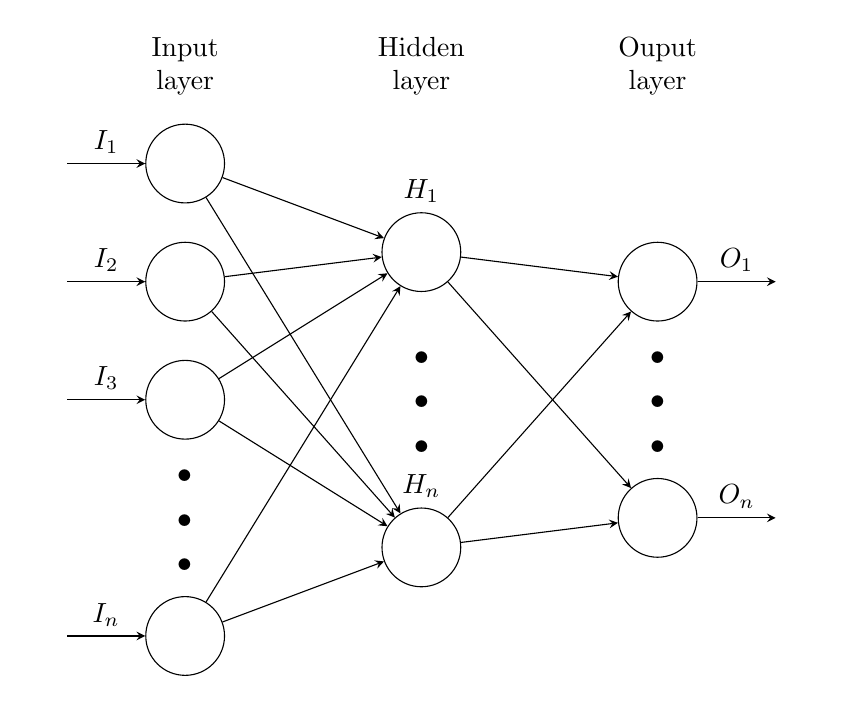
\begin{tikzpicture}[x=1.5cm, y=1.5cm, >=stealth]

\foreach \m/\l [count=\y] in {1,2,3,missing,4}
  \node [every neuron/.try, neuron \m/.try] (input-\m) at (0,2.5-\y) {};

\foreach \m [count=\y] in {1,missing,2}
  \node [every neuron/.try, neuron \m/.try ] (hidden-\m) at (2,2-\y*1.25) {};

\foreach \m [count=\y] in {1,missing,2}
  \node [every neuron/.try, neuron \m/.try ] (output-\m) at (4,1.5-\y) {};

\foreach \l [count=\i] in {1,2,3,n}
  \draw [<-] (input-\i) -- ++(-1,0)
    node [above, midway] {$I_\l$};

\foreach \l [count=\i] in {1,n}
  \node [above] at (hidden-\i.north) {$H_\l$};

\foreach \l [count=\i] in {1,n}
  \draw [->] (output-\i) -- ++(1,0)
    node [above, midway] {$O_\l$};

\foreach \i in {1,...,4}
  \foreach \j in {1,...,2}
    \draw [->] (input-\i) -- (hidden-\j);

\foreach \i in {1,...,2}
  \foreach \j in {1,...,2}
    \draw [->] (hidden-\i) -- (output-\j);

\foreach \l [count=\x from 0] in {Input, Hidden, Ouput}
  \node [align=center, above] at (\x*2,2) {\l \\ layer};

\end{tikzpicture}


\subsection{Including Code}

\begin{lstlisting}[language=Python]
        def hello_world_python():
            print("Hello floating world!")
\end{lstlisting}

% using R
%\begin{lstlisting}[language=R]
%hello_world_R <- function() {
%  print("Hello floating world!")
%}
%\end{lstlisting}

% using bash
%\begin{lstlisting}[language=bash]
%hello_world_bash() {
%  echo "Hello floating world!"
%}
%\end{lstlisting}

% using MATLAB
%\begin{lstlisting}[language=Matlab]
%function hello_world_matlab()
%  disp('Hello floating world!');
%end
%\end{lstlisting}


\subsection{Including Chemistry}

\begin{center}
	\chemfig{*6((=O)-N(-H)-(*5(-N=-N(-H)-))=-(=O)-N(-H)-)}
\end{center}

\subsection{Including Circuits} \nopagebreak

\begin{figure}[!hb] % h means here. t: top, b: bottom 
  \begin{center}
    \begin{circuitikz}
      \draw (0,0)
      to[V,v=$U_q$] (0,2) % The voltage source
      to[short] (2,2)
      to[R=$R_1$] (2,0) % The resistor
      to[short] (0,0);
    \end{circuitikz}
    \caption{Circuit 1.}
  \end{center}
\end{figure}

\FloatBarrier

\newpage
\thispagestyle{empty}
\section{Including an Article}

\includepdfset{pagecommand=\thispagestyle{scrheadings}} % adds page numbers to imported pdfs
\includepdf[pages=1-3, pagecommand={\pagestyle{empty}}]{pdfs/curie_notes.pdf}
